% =====================================================================
%  Entregable T2(b): Evolucion temporal por accion del exponencial (Krylov)
%  Fragmento \input-able en context/doc/mpemba_cuantico.tex
% =====================================================================
\section{Evolución temporal (b): acción del exponencial por Krylov}
\label{sec:t2b}

\subsection{Explicación del framework}
El método~(b) resuelve la misma evolución $\dot\rho=\mathcal{L}[\rho]$ pero por una
vía distinta: en lugar de integrar paso a paso, aproxima directamente la
\textbf{acción del exponencial del Liouvilliano},
\[
\rho(t+\tau)=e^{\tau\mathcal{L}}[\rho(t)],
\]
que es la solución \emph{exacta} en un paso de tamaño $\tau$. La dificultad es que
$e^{\tau\mathcal{L}}$ es un objeto de dimensión $d^2\times d^2$ imposible de
formar. La idea de Krylov es proyectar la acción sobre el subespacio
$\mathcal{K}_m=\text{span}\{\rho,\mathcal{L}\rho,\dots,\mathcal{L}^{m-1}\rho\}$,
de dimensión $m\ll d^2$, donde el exponencial es trivial de calcular.

\subsection{Del modelo teórico a la discretización (paso a paso)}
\label{ssec:t2b_discr}

\paragraph{Paso 0 — Modelo teórico.} El mismo de~(a): la ecuación maestra GKSL
$\dot\rho=\Lop[\rho]$ para la cadena de Ising disipativa (Hamiltoniano $H$ y
canales $L_\mu$ idénticos, \S\ref{ssec:t2a_discr}).

\paragraph{Paso 1 — Solución formal exacta.} En lugar de integrar la EDO, se usa
que la solución del PVI es \emph{exacta} en un paso de tamaño $\tau$ mediante el
exponencial del generador:
\[
\rho(t+\tau)=e^{\tau\Lop}[\rho(t)].
\]
El obstáculo: $e^{\tau\Lop}$ vive en el superoperador de dimensión
$d^2\times d^2$, imposible de formar y exponenciar para $N$ grande.

\paragraph{Paso 2 — Discretización por proyección de Krylov (Arnoldi).} Se proyecta
la acción del exponencial sobre el subespacio de Krylov
$\mathcal{K}_m=\text{span}\{\rho,\Lop\rho,\dots,\Lop^{m-1}\rho\}$ ($m\ll d^2$). Con
\textbf{Arnoldi} se construye una base ortonormal $\{Q_0,\dots,Q_{m-1}\}$ (cada
$Q_i$ es un operador $d\times d$; producto interno de Frobenius
$\langle A,B\rangle=\Tr(A^\dagger B)$) y la matriz de Hessenberg
$H_m\in\mathbb{C}^{m\times m}$ que representa $\Lop$ en esa base. El \emph{único}
ingrediente que toca el sistema grande es la acción $w=\Lop[Q_j]$ en cada
iteración de Arnoldi.

\paragraph{Paso 3 — Exponencial pequeño y reconstrucción.} La acción discretizada es
\[
e^{\tau\Lop}[\rho]\;\approx\;\|\rho\|_F\;\sum_{i=0}^{m-1}\big[e^{\tau H_m}\big]_{i,0}\,Q_i,
\]
con $e^{\tau H_m}$ calculado sobre la matriz \emph{pequeña} $m\times m$ por
\emph{scaling-and-squaring} con serie de Taylor (\texttt{small\_expm}). Coste por
bloque: $m$ aplicaciones de $\Lop$ (Arnoldi) $+\,\mathcal{O}(m\,d^2)$ y un
$e^{\tau H_m}$ de coste $\mathcal{O}(m^3)$ despreciable. La ventaja decisiva: para
$\tau$ dentro del radio de convergencia, $m\sim20$--$30$ basta para precisión de
máquina y \emph{un solo bloque avanza un paso de tiempo grande}.

\subsection{Implementación serial y líneas de código}
En \texttt{b\_accion\_exponencial/src/krylov\_evolution.cpp}. El bucle de Arnoldi
(Paso~2) es el corazón del método; nótese que cada iteración llama a la misma
acción \texttt{apply\_lindblad} de~(a) —es decir, \emph{comparte el hotspot
paralelizable}—:

\begin{lstlisting}[language=C++,caption={Bucle de Arnoldi de \texttt{krylov\_step} (\texttt{krylov\_evolution.cpp}): la línea \texttt{apply\_lindblad(...)} es la acción matrix-free de $\mathcal L$, donde se cuenta el trabajo (\texttt{L\_applies}) y donde reside la paralelización OpenMP (vía \texttt{matmul}, Listado~\ref{lst:t2b_omp}).},label={lst:t2b_arnoldi}]
for (int j = 0; j < m; ++j) {
    Mat w = apply_lindblad(H, Ls, Lds, LdL, Q[j], d); ++L_applies;   // <-- hotspot (OpenMP)
    for (int i = 0; i <= j; ++i) {                       // ortogonalizacion de Gram-Schmidt
        cd hij = fro_dot(Q[i], w); Hess[i*m+j] = hij; axpy(w, Q[i], -hij);
    }
    double hj = fro_norm(w);
    Hess[(j+1)*m+j] = hj;
    if (hj < 1e-12) { mm = j + 1; break; }               // convergencia anticipada
    Q.push_back(scaled(w, 1.0 / hj));
}
\end{lstlisting}

\subsection{La directiva de paralelización (OpenMP)}
El \emph{hotspot} es el mismo que en~(a): el producto de matrices densas, llamado
$m$ veces por bloque dentro de \texttt{apply\_lindblad}. La directiva es por tanto
idéntica —una sola \texttt{\#pragma omp parallel for} en \texttt{matmul}
(\texttt{common/lindblad.hpp})—, lo que explica que el escalado paralelo de~(b)
sea equivalente al de~(a):

\begin{lstlisting}[language=C++,caption={La misma directiva OpenMP que en T2(a): el bucle de filas de \texttt{matmul} es el único punto paralelizado (compartido por RK4 y Krylov).},label={lst:t2b_omp}]
    #pragma omp parallel for schedule(static)   // <-- DIRECTIVA: filas i repartidas entre hilos
    for (int i = 0; i < d; ++i)
        for (int k = 0; k < d; ++k) { /* C[i,:] += A[i,k] * B[k,:] */ }
\end{lstlisting}

\subsection{Justificación de la paralelización: OpenMP}
Como en el método~(a), el \emph{hotspot} es la acción $\mathcal{L}[\cdot]$ (el
producto de matrices densas), llamada $m$ veces por bloque. La ortogonalización
de Arnoldi añade productos internos de Frobenius de coste $\mathcal{O}(d^2)$,
mucho menores que el $\mathcal{O}(d^3)$ del \texttt{matmul}. Por tanto el patrón
sigue siendo de \textbf{memoria compartida} dominado por \texttt{matmul}, y el
paradigma natural vuelve a ser \textbf{OpenMP} sobre el mismo bucle. (En el
régimen de muchos cuerpos, donde $d^2$ no cabe en memoria, la acción de Krylov se
paraleliza con MPI distribuyendo el vector $\ket{\rho}\rangle$; aquí, con $\rho$
denso en un nodo, OpenMP es lo adecuado.) La corrección se verifica de dos formas:
serial y paralelo dan el mismo resultado, y el resultado coincide con el del
método~(a) (RK4) a todas las cifras: $D_{HS}^{\text{final}}=0{,}4241128226$ para
$N=6$, idéntico por ambos métodos (referencia exacta por evolución espectral:
$D_{HS}^{\text{exacto}}=0{,}42411283$).

\subsection{Comparación serial vs paralelo}
\begin{figure}[h]
\centering
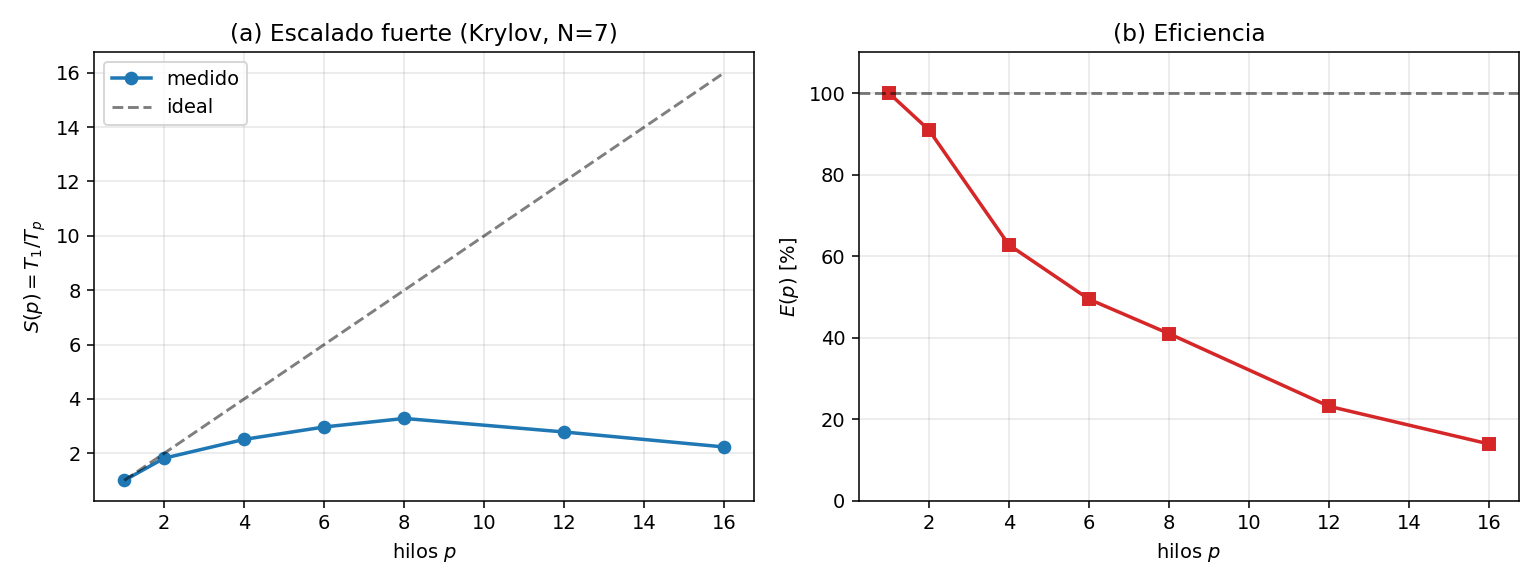
\includegraphics[width=0.92\textwidth]{../../T2/b_accion_exponencial/results/fig_t2b_speedup.png}
\caption{Escalado fuerte del método de Krylov (Ising disipativo $N=7$, $d=128$).
El comportamiento es análogo al del método~(a): speedup sublineal que satura en
los núcleos físicos, por las mismas causas (fork/join del \texttt{matmul},
\emph{memory-bandwidth bound}, hyperthreading sin ancho de banda extra). Pico
$S_{\max}\approx3{,}3$, eficiencia $41\,\%$ a 8 hilos (ligeramente mejor que
RK4: hay menos llamadas a \texttt{matmul} por unidad de trabajo).}
\label{fig:t2b_speedup}
\end{figure}

La Figura~\ref{fig:t2b_serial_parallel} muestra la mejora de forma directa: el
\textbf{tiempo de cómputo en serie (1~hilo) frente al paralelo (8~hilos)} en
función del tamaño del sistema~$N$ (malla $d=2^N$), a igual paso $\tau$ y misma
dimensión de Krylov $m$. Igual que en~(a), las dos curvas crecen como $\sim d^3$
y el hueco entre ellas —la ganancia— se ensancha con la malla.

\begin{figure}[h]
\centering
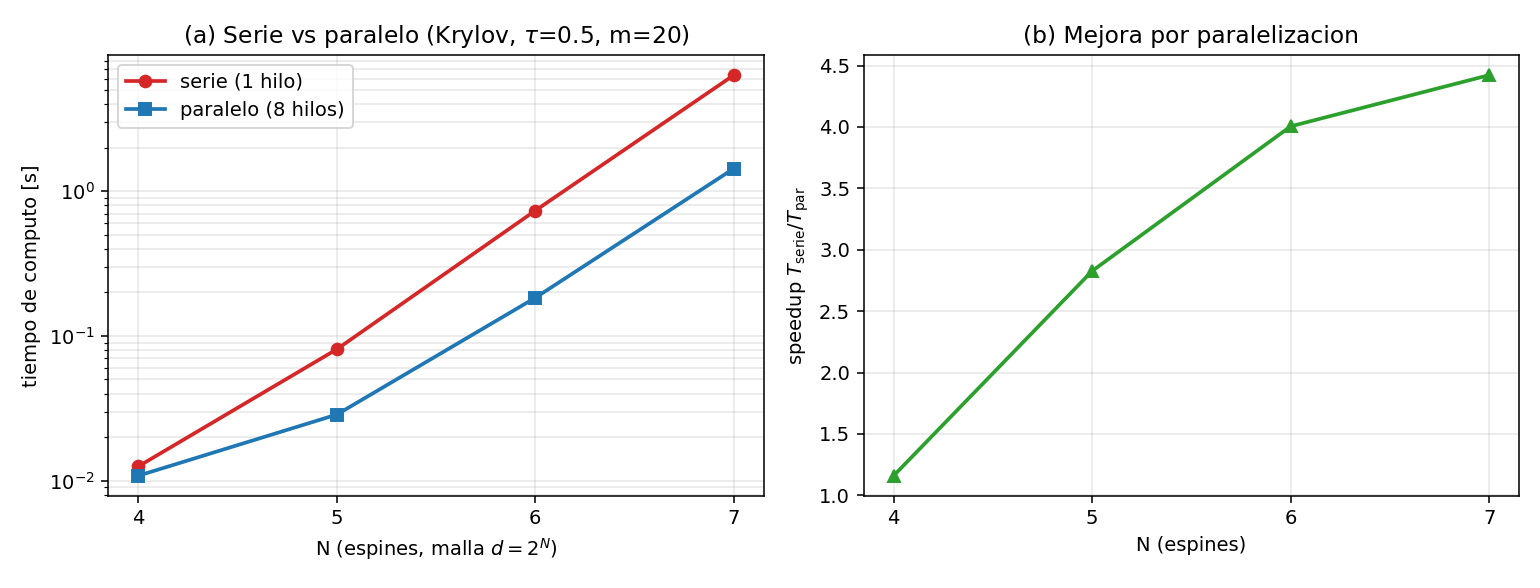
\includegraphics[width=0.92\textwidth]{../../T2/b_accion_exponencial/results/fig_t2b_serial_parallel.png}
\caption{Tiempo de cómputo \textbf{serie vs paralelo} del método de Krylov frente
al tamaño del sistema $N$ (malla $d=2^N$), a $\tau=0{,}5$ y $m=20$ fijos.
(a)~curvas de $1$~hilo (rojo) y $8$~hilos (azul) en escala log; (b)~speedup
$T_{\mathrm{serie}}/T_{\mathrm{par}}$ resultante. El patrón es el mismo que el de
RK4 porque el hotspot paralelo —el \texttt{matmul} de la acción de $\mathcal L$—
es común a ambos métodos.}
\label{fig:t2b_serial_parallel}
\end{figure}

\subsection{Comparación de método (a vs b): el resultado central}
La ventaja de Krylov no está en el escalado paralelo (idéntico al de RK4) sino en
el \textbf{trabajo necesario para una precisión dada}. La
figura~\ref{fig:t2b_method} mide el error del observable $D_{HS}$ final frente a
una referencia de alta precisión, en función del número de aplicaciones de
$\mathcal{L}$ (la operación cara, independiente de la máquina):

\begin{figure}[h]
\centering
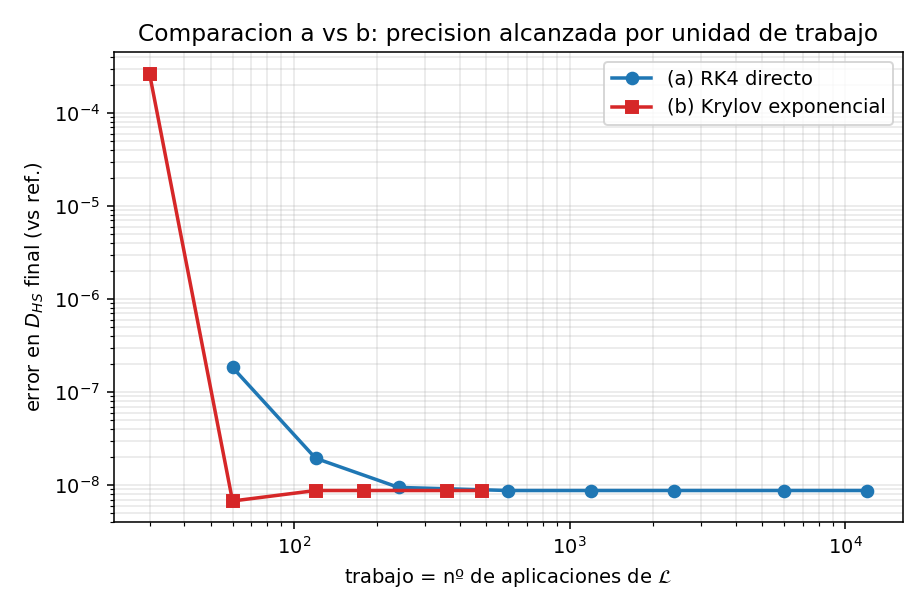
\includegraphics[width=0.7\textwidth]{../../T2/b_accion_exponencial/results/fig_t2b_method_compare.png}
\caption{Error del observable $D_{HS}$ final frente a la referencia exacta
(evolución espectral), en función del trabajo. \textbf{A igual trabajo
($\approx 60$ aplicaciones de $\mathcal{L}$), Krylov es $\sim$25$\times$ más
preciso} ($7\times10^{-9}$ frente a $2\times10^{-7}$ de RK4). El punto Krylov de
$m=10$ (no convergido, $2\times10^{-4}$) cae cinco órdenes de magnitud al pasar a
$m=20$: convergencia \emph{super-algebraica} en $m$, frente a la algebraica
($\propto\Delta t^4$) de RK4. El suelo $\sim 9\times10^{-9}$ es la precisión de
la propia referencia.}
\label{fig:t2b_method}
\end{figure}

La interpretación física/numérica: RK4 converge \emph{algebraicamente} (el error
baja como $\Delta t^4$), mientras que Krylov converge \emph{super-algebraicamente}
(casi exponencial en $m$) porque captura la acción exacta del exponencial dentro
del subespacio. En este sistema disipativo \emph{no rígido}, ambos métodos son de
trabajo comparable para precisiones moderadas, pero Krylov presenta tres ventajas
estructurales: (i)~a igual trabajo es $\sim$25$\times$ más preciso; (ii)~usa pasos
de tiempo $5\times$ mayores ($\tau=1{,}0$ frente a $\Delta t=0{,}2$) manteniéndose
estable y exacto; (iii)~es \textbf{incondicionalmente estable}, mientras que RK4
tiene un límite de estabilidad $\Delta t<2{,}8/|\lambda_{\max}|$. Esta ventaja se
vuelve \emph{decisiva} para generadores \emph{rígidos} (escalas de energía grandes
o disipación fuerte) y para alcanzar el estado estacionario, donde el límite de
estabilidad obliga a RK4 a dar muchísimos pasos diminutos. RK4 sigue siendo
preferible cuando se necesita la trayectoria \emph{densamente} muestreada en el
tiempo o cuando el Liouvilliano depende del tiempo.

\subsection{Resultados y conclusión del método (b)}
La figura~\ref{fig:t2b_relax} muestra la curva de relajación obtenida con pasos
\emph{grandes} ($\tau=0{,}25$), inalcanzables para RK4 a esa precisión. Resumen de
la comparación a--b:
\begin{itemize}[leftmargin=1.6em,itemsep=1pt]
\item Misma física (resultados idénticos), misma paralelización (OpenMP sobre
\texttt{matmul}, escalado sublineal equivalente).
\item Krylov~(b): mucho menos trabajo para alta precisión y pasos de tiempo
grandes; ideal para llegar al estacionario o muestrear pocos tiempos.
\item RK4~(a): más simple, robusto, y mejor para trayectorias densas o
generadores dependientes del tiempo.
\end{itemize}

\begin{figure}[h]
\centering
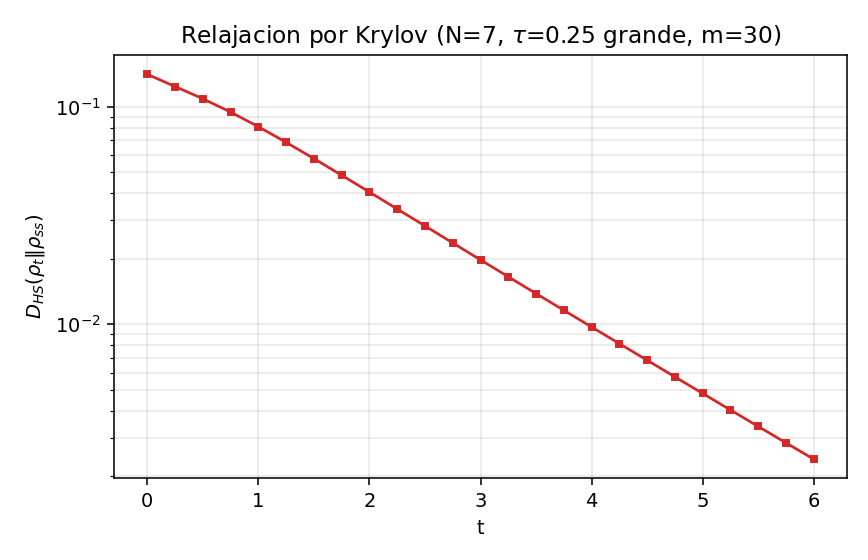
\includegraphics[width=0.6\textwidth]{../../T2/b_accion_exponencial/results/fig_t2b_relax.png}
\caption{Relajación $D_{HS}(t)$ por Krylov con pasos grandes $\tau=0{,}25$
($N=7$), medida al \textbf{estado estacionario verdadero} $\rss$ (núcleo de
$\Lop$): por eso baja a $0$.}
\label{fig:t2b_relax}
\end{figure}

\subsection{El efecto Mpemba: cruce de curvas}
El método de Krylov reproduce el efecto Mpemba con idéntica física que RK4 (ambos
resuelven la misma ecuación maestra). La Figura~\ref{fig:t2b_mpemba} evoluciona por
Krylov dos preparaciones del mismo Ising disipativo: $\ket{+}^{\otimes N}$ (parte
lejos) y $\ket{0}^{\otimes N}$ (parte cerca), midiendo la distancia al estado
estacionario verdadero $\rss$. La que parte lejos \textbf{adelanta} a la otra en
$t^*\approx0{,}69$ —el mismo $t^*$ que da RK4 (\S\ref{sec:t2a}), confirmando que el
cruce es físico y no del integrador.

\begin{figure}[h]
\centering
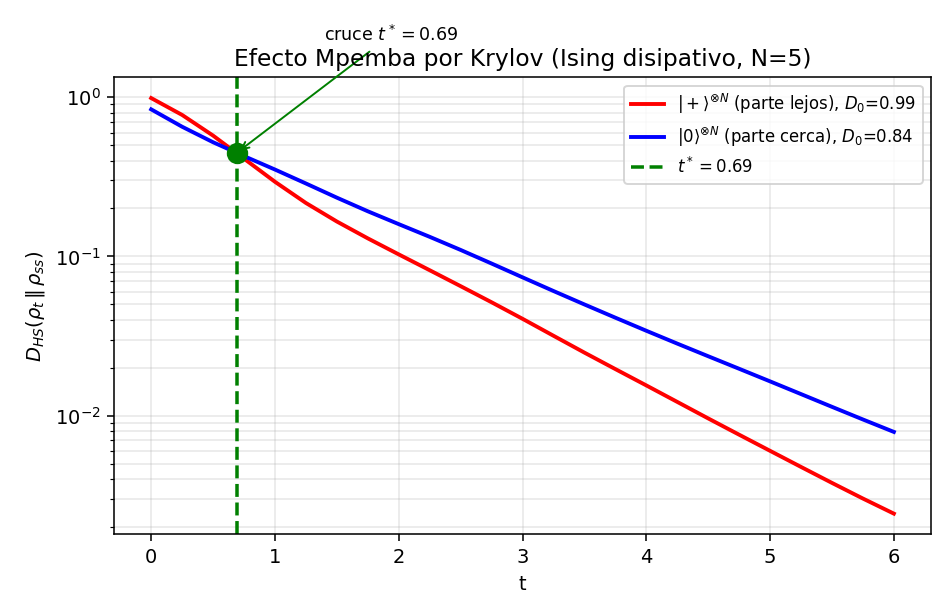
\includegraphics[width=0.72\textwidth]{../../T2/b_accion_exponencial/results/fig_t2b_mpemba.png}
\caption{Efecto Mpemba por Krylov (Ising disipativo, $N=5$). $D_{HS}(t)$ a $\rss$
para $\ket{+}^{\otimes N}$ (roja, lejos) y $\ket{0}^{\otimes N}$ (azul, cerca): la
roja cruza a la azul en $t^*\approx0{,}69$, idéntico al de RK4.}
\label{fig:t2b_mpemba}
\end{figure}
